\section{函数与极限}

\subsection{复习要点}

\subsubsection{预备知识}

\setstretch{1.75}

\textbf{1.~~反三角函数}\vspace{0.5em}

严格来说，反三角函数并不是三角函数的反函数.
以$y=\arcsin x$为例，
它的函数值$y$由$x = \sin y$给出.
但是，$y = \sin x$的一个函数值$y$可以对应多个$x$
（即$y = \sin x$不是$\mathbb{R}\to \mathbb{R}$的单射），
所以不能定义反函数.
解决方案很简单，
就是只取$\mathbb{R}$的某段区间.
例如取$x \in \left[ -\frac{\pi}{2},~\frac{\pi}{2} \right] $，
$y = \sin x$在该区间上是单调递增的，
存在反函数，便将其定义为$\arcsin$.
事实上，这样的区间取法有很多，
例如$\left[ \frac{\pi}{2},~\frac{3\pi}{2} \right] $，
$\left[ \frac{3\pi}{2},~\frac{5\pi}{2} \right]$等等都是可行的.
但是，
取$\left[ -\frac{\pi}{2},~\frac{\pi}{2} \right] $来定义反正弦函数
（即规定$\arcsin$的值域是$\left[ -\frac{\pi}{2},~\frac{\pi}{2} \right] \vphantom{\frac{\frac{1}{1}}{1}}$）
是最简明的，也是约定俗成的做法.
因此，我们在使用反三角函数时也要遵守这些约定.

接下来，我们介绍三个反三角函数的基本性质，建议熟记：\vspace{0.5em}

（1）$y = \arcsin x$：定义域为$[-1,~1]$，值域为$\left[ -\frac{\pi}{2},~\frac{\pi}{2} \right]$，
奇函数，在定义域内单调递增.

（2）$y = \arccos x$：定义域为$[-1,~1]$，值域为$[0,~\pi]$，
函数图像有一对称中心$\left( 0,~\displaystyle\frac{\pi}{2} \right)$，
在定义域内单调递减.

（3）$y = \arctan x$：定义域为$\mathbb{R}$，
值域为$\left( -\frac{\pi}{2},~\frac{\pi}{2} \right)$，
奇函数，$y =\displaystyle\frac{\pi}{2}$
和$y =-\displaystyle\frac{\pi}{2}$是其两条水平渐近线，
在定义域内单调递增.\vspace{0.5em}

在使用反三角函数时，请同学们务必注意定义域和值域.
在以下三例中，不多加小心就很容易犯错：\vspace{0.5em}

（1）不能认为$\arcsin (\sin x)$和$x$没区别.
因为$x$可能不在$\arcsin$的值域内.

（2）不能由诱导公式认为$\arccos x = -\arccos(-x)$，
正确的等式是$\arccos x = \pi -\arccos(-x)$.

（3）根据两角和公式，
似乎可以推出$\arctan x+\arctan y=\arctan \left( \displaystyle\frac{x+y}{1-xy} \right)$.
但这其实也不一定对，
因为$\arctan x+\arctan y$的值可能超过了$\displaystyle\frac{\pi}{2}$，那就超出了$\arctan$的值域.\vspace{1em}

\textbf{2.~~其他需要关注的预备知识}

熟悉符号函数$y =$ sgn$x$,高斯取整函数$y = [x]$和狄利克雷函数的定义.
另外，也可以了解一下黎曼函数：

\[
\setstretch{1.25}
y = R(x)=
\begin{cases}
\displaystyle\frac{1}{p} &\quad x = \frac{q}{p} \in (0, 1),~~p,q\text{为互素的正整数}
\\
0 &\quad x \in [0, 1]\setminus \mathbb{Q} \\
1 &\quad x = 0~\text{或}~1\\
\end{cases}
\] \setstretch{1.75}

黎曼函数的特殊性质是：在有理点处为可去间断点，在无理点处连续.
证明可作为习题（见例\ref{ex:ch01-04}）.

另外，需要熟悉映射的相关概念，尤其是\textbf{单射}、\textbf{满射}和\textbf{双射}的关系.
有几点提示同学们：
（1）\textbf{像集合}就是我们一般所说的“值域”，它不是指“$E \to F$”的那个集合$F$.
（2）一个映射是\textbf{双射}（或称\textbf{可逆映射}），当且仅当它既是\textbf{单射}又是\textbf{满射}.不熟悉映射的同学可以围绕这句话来理解概念.
（3）北大版教材中，“一一映射”是“单射”的另一种说法.
但在别的许多教材中，“一一映射”与“双射”是同义词.

\subsubsection{极限和连续的定义}

同学们一方面需要对“极限为什么要这样定义”有直观的认识，而不是死背定义（北大版教材中讲解得比较好）；
另一方面，也要能熟练写出定义，
否则无法做相关的证明题.
不仅如此，还要会写它的否定形式：
从形式上来说，
只要把极限定义中的“任意”改为“存在”，
“存在”改为“任意”，然后改变不等号的方向即可.
写下来就是：\vspace{0.5em}

\textit{设$\left \{ a_{n} \right \}$是一个给定的序列. 对于任意给定的自然数$N$，若存在正数$\epsilon$，使得存在一个$n>N$，满足$|a_{n}-l|\ge \epsilon$，则$\left \{ a_{n} \right \}$的极限不存在.}

\vspace{0.5em}

对于这个否定形式的叙述，我们也可以直观地理解：
假设我们猜测$\left \{ a_{n} \right \}$的极限是$l$，
然而却发现，无论顺着$\left \{ a_{n} \right \}$往后找多少项，
总能找到一些捣乱分子上下乱窜，
跳出$(l-\epsilon,~l+\epsilon)$的限制，
那么显然$\left \{ a_{n} \right \}$不可能是“无限趋向$l$”的，
我们就可以说$\left \{ a_{n} \right \}$的极限不是$l$.
如果我们猜了一圈，
都没有发现合适的$l$和$\epsilon$能把所有的捣乱分子都限制住，
那么$\left \{ a_{n} \right \}$的极限就不存在.

由此我们可以发现，利用定义的否定形式证明$a_{n}$的极限不是某个给定的$l$
是较为简单的——我们只需要指出捣乱分子具体是谁即可.
但是，用定义法证明“$\left \{ a_{n} \right \}$的极限不存在”却比较难，
因为我们不可能真的去尝试所有的$l$.
之后我们会介绍证明极限不存在的其他方法.\vspace{0.5em}

函数在无穷远处的极限，与序列的极限类似，这里不再赘述.
但是对于函数在某点处的极限，
初学时或许会不习惯.
以$f(x) = \sqrt{3x+1}$为例，
有同学可能会问，直接将$x=1$代入$f(x)$，不就算出$2$这个答案了吗，
何必大费周章地用$\epsilon\text{-}\delta$语言去证明呢？
相信在学习了函数连续的概念之后，
同学们都能回答这个问题了：
刚才那位同学是默认了这个函数是连续的，
才能直接通过函数值来计算极限.
这其中存在着逻辑问题
——我们还没有证明函数的极限存在，
怎么知道它连续呢？
试想，如果将题目中的函数改成：
\[
\setstretch{1.25}
f(x)=
\begin{cases}
\sqrt{3x+1} &\quad x \ne 1
\\[2pt]
100 &\quad x = 1
\end{cases}
\] \setstretch{1.75}
那位同学又将如何应对？

借这个例子，我们强调，
函数的“美好”性质是根据“极限存在$\to$连续$\to$可导”的顺序建立起来的，在没有证明前者的情况下，
我们不能假定后者成立.
某些证明题会给出一些“身份不明”的函数$f(x)$.
我们应该不惮以最坏的恶意揣测这些出题人随手抛出的函数——
只要题目没说它可导，我们就不能对它求导；
只要题目没说它连续，我们就不能利用连续的相关性质.\vspace{0.5em}

总结起来，函数在某点处的极限，
是我们根据该点左侧和右侧的变化趋势来对该点函数值做出的“预测”.
这种预测单看左侧或者单看右侧也能做出来（\textbf{左极限}和\textbf{右极限}），
但是只有两个方向的预测结果相吻合（左右极限相等），我们才认为给出了一个明确的预测结果（极限存在）. 当然，这个预测结果可能与函数在该点处的实际函数值不符.
但如果恰好相符，我们就说函数在该点是连续的.
这条主线就是本章的核心精神.

\subsubsection{极限相关结论和定理}

\textbf{1.~~单调有界原理}：
\textit{单调递增有上界则极限存在；
单调递减有下界则极限存在.}

在北大版教材中，单调有界原理作为刻画实数域完备性的一种说法出现.
据此，在我们的高数课程中可以把它当作公理使用，不需要证明.\vspace{0.5em}

\textbf{2.~~极限的唯一性}：见本讲义例\ref{ex:ch01-02}.\vspace{0.5em}

\textbf{3.~~极限不等式}：见教材1.3节定理2、定理3；1.4节定理4.\vspace{0.25em}

需要注意的是，当数列$\left \{ a_{n} \right \}$的每一项都严格大于$\left \{ b_{n} \right \}$的每一项时，
不能推出$\lim\limits_{n \to \infty}a_{n} > \lim\limits_{n \to \infty}b_{n}$，
因为可能存在$\lim\limits_{n \to \infty}a_{n} = \lim\limits_{n \to \infty}b_{n}$的情况.\vspace{0.5em}

\textbf{4.~~夹逼定理}：见教材1.3节定理1，1.4节定理1.\vspace{0.5em}

\textbf{5.~~极限的四则运算}：见教材1.3节定理4、定理3；1.4节定理2.\vspace{0.5em}

\textbf{6.~~收敛序列/函数的子列收敛}：见教材1.3节定理5、定理3；1.4节定理5.\vspace{0.5em}

\textbf{7.~~两个重要极限}

（1）$\lim\limits_{x \to 0}\frac{\sin x}{x} = 1$ （教材1.4节，夹逼定理的例题）\par
（2）自然常数$e$ （教材1.3节例题，数列版本，用单调有界原理证明；
教材1.4节例题，函数版本，用夹逼定理证明）\par
\par \vspace{1em}

以下带星号的内容在课本上没有出现，但是理解难度不高，也建议了解并运用在证明过程里.
这些结论的证明方法本身也可以当作练习题.\vspace{0.5em}

*\textbf{8.~~有界性}\vspace{0.25em}

\textbf{收敛序列的有界性}~~\textit{如果数列$\left \{ x_{n} \right \}$收敛，那么数列$\left \{ x_{n} \right \}$有界.}

\textbf{收敛函数的局部有界性}~~\textit{如果函数$f(x)$在$x_{0}$处的极限存在，那么存在常数$M>0$和$\delta >0$，
使得当$0<|x-x_{0}|<\delta$时，有$|f(x)|\le M$.}

证明用到了分段处理的技巧. （收敛序列的有界性证明见讲义例\ref{ex:ch01-05}）\vspace{0.5em}

*\textbf{9.~~保号性}\vspace{0.25em}

\textbf{序列极限的保号性}~~\textit{如果$\lim\limits_{n \to \infty}x_{n}=a$，且$a>0$（或$a<0$），
那么存在正整数$N$，当$n>N$时，都有$x_{n}>0$（或$x_{n}<0$）.}

\textbf{函数极限的局部保号性}~~\textit{如果$\lim\limits_{x \to x_{0}}f(x)=a$，且$a>0$（或$a<0$），
那么存在$\delta>0$，当$0<|x-x_{0}|<\delta$时，都有$f(x)>0$（或$f(x)<0$）.}
（序列极限的保号性证明见讲义例\ref{ex:ch01-03}）\vspace{0.5em}

以上两个定理是极限不等式的推广情况，但是更加清楚地体现序列（函数）的极限会限制其在无穷远（收敛点附近）的行为.
例如对于收敛序列，
它的前$100$，$1000$乃至任意的前$N$项都可以很“狂放”，
但是只要把范围限定在足够远，
序列就会变得十分“老实”，不再产生大的波动.
这个波动的振幅可以通过选取足够大的$N$控制在$|a|$之内.\vspace{0.5em}

*\textbf{10.~~柯西收敛原理}\vspace{0.25em}

\textbf{数列的柯西收敛原理}~~\textit{数列$\left \{ x_{n} \right \}$收敛的充要条件是：对于任意的$\epsilon>0$，存在正整数$N$，
使得当$n$、$m>N$时，有$|x_{n}-x_{m}|<\epsilon$.}

柯西收敛原理的优越之处在于，
不需要指出极限值$l$具体是谁就能判断一个数列是否收敛.
教材将其放在级数章节中讲述.
我们在这里介绍这个定理，
是希望同学们学习一种思路：
判断一个序列的极限是否存在，
除了研究通项公式之外，
项与项之间的关系也能提供一些线索.
在1.2节将针对这个思路进行讲解.

\subsubsection{函数连续相关结论和定理（教材1.5节）}
\textbf{1.~~复合函数的连续性}：\textit{连续函数的复合依然是连续函数.}\par
\textbf{2.~~反函数的连续性}：\textit{连续函数的反函数是连续函数.}\par
\textbf{3.~~初等函数的连续性}：\textit{初等函数在其定义域的每个子区间内都是连续函数.}\par
*\textbf{4.~~Lipschitz条件}：见教材1.5节例题2\par

\subsubsection{间断点的分类（教材1.5节最后一部分）}\par
北大版教材的叙述较为简单.
这里参考其他教材的说法，
补充说明间断点相关的定义和概念，帮助同学们整理. \par

若函数$f(x)$在$x_{0}$的去心邻域内
（即存在常数$\delta>0$，使得在$(x_{0}-\delta,~x_{0})\cup(x_{0},~x_{0}+\delta)$内）有定义，
且在$x_{0}$处不连续，则称$x_{0}$是$f(x)$的\textbf{间断点}. 注意，定义并没有要求$f(x)$在$x_{0}$处有定义. 而且，教材中所讲的间断点的分类方法，与$f(x)$在$x_{0}$处是否有定义无关.\par

在此基础上，若$f(x)$在$x_{0}$处的左右极限都存在，则称$x_{0}$为\textbf{第一类间断点}. 第一类间断点又分两类：若左右极限不相等，称为\textbf{跳跃间断点}；
若左右极限相等，则称为\textbf{可去间断点}.

不是第一类间断点的，都是\textbf{第二类间断点}. 第二类间断点也分两类：
若$f(x)$从$x_{0}$的左侧或右侧趋向无穷（从而左极限或右极限不存在），则称$x_{0}$为\textbf{无穷间断点}；
若$f(x)$在$x_{0}$左侧或右侧有界，
但是因为振荡而导致左极限或右极限不存在
（例如$\sin \frac{1}{x}$在$x=0$处的情形），
则称$x_{0}$为\textbf{振荡间断点}.

与教材中相比，这里给出的分类方法更加完全（尽管理论上还存在诸如左侧振荡右侧无穷的离谱间断点）.
理解上述概念之后，
就不必担心还存在其他“不可名状”的间断点类型.
若考试题目要求判断间断点类型，
推荐完整地写上两级分类（例如：第一类间断点，可去间断点）.\vspace{0.5em}

注：间断点的定义存在一些争议.
在上文的定义中，
要求$f(x)$在$x_{0}$的“左右附近”有定义，
这看似滴水不漏，实则也会造成一些问题.
例如，设符号函数sgn$(x)$的定义域为$\mathbb{R}$，
则$x=0$是间断点；
然而，
若将其限制在区间$(-\infty,~0]$上，
则$x=0$就不是间断点，
因为函数在$x>0$处没有定义.
这就显得很不讲道理了.
北大版教材可能为了避免讨论这样的问题，
只是模糊地要求$f(x)$在$x_{0}$的“附近”有定义.
既然如此，我们也就不必纠结这种细枝末节的问题了.

\subsubsection{闭区间上连续函数的性质（教材1.6节）}\par
学习这部分的知识要注意两点：
第一，不能默认题目所给的函数$f(x)$都是连续的，也不能认为“闭区间”是一个无关紧要的条件.
对于本节的所有定理，当函数不连续或者指定区间为开区间时都存在反例.
第二，本节的定理并不是函数连续的充要条件，例如，不是所有具有介值性的函数都是连续函数. \vspace{0.5em}

\textbf{1.~~介值定理}~~\textit{若$f(x)$是$[a,b]$上的连续函数，
对于$f(a)$和$f(b)$之间的任意一个值$\eta$，都存在$\xi \in [a,b]$，使得$f(\xi) = \eta$.}

\textbf{2.~~最值定理}~~\textit{闭区间上的连续函数一定存在最大值和最小值.}

\textbf{3.~~有界性定理}~~\textit{闭区间上的连续函数一定存在上下界.}

\subsubsection{无穷大量与无穷小量}

当$n \to \infty$时，常见的无穷大量比较关系如下（“$\ll$”表示“远小于”，即后者是前者的高阶无穷大量）：
$$
\ln n \ll n^k \ll a^{n} \ll n! \ll n^n
$$
其中$k>0$，$a>1$.

记住以上关系，可以猜出题目中某些极限的值，并且有助于想到证明方法. 前提是上述关系必须要会自己证明.
另外，今后在学习反常积分和级数的相关知识时，能够快速估计无穷大量“究竟有多大”，也是对学习很有帮助的.\vspace{0.5em}

对上述的无穷大量取倒数，就得到了一系列无穷小量的关系：
$$
\frac{1}{\ln n} \gg \frac{1}{n^k} \gg \frac{1}{a^{n}} \gg \frac{1}{n!} \gg \frac{1}{n^n}
$$

接下来列出一些等价无穷小的关系（当$x \to 0$时），同学们可依据自身情况选择背诵一些：
\begin{gather*}
    \sin x\sim x~~~~~~~\tan x\sim x~~~~~~~\ln(1+x)\sim x~~~~~~~ e^{x}-1\sim x \\
    \arcsin x\sim x~~~~~~~\arctan x\sim x~~~~~~~ \log_{a}(1+x) \sim \frac{x}{\ln a}~~~~~~~x - \ln(1+x) \sim \frac{x^{2}}{2} \\
    1-\cos x\sim \frac{x^{2}}{2}~~~~~~~\ln(x+\sqrt{1+x^{2}})\sim x~~~~~~~x-\sin x\sim \frac{x^{3}}{6} ~~~~~~~\tan x-x \sim \frac{x^{3}}{3}\\
    (1+x)^{\alpha} - 1 \sim \alpha x~~~~~~~\arcsin x-x \sim \frac{x^{3}}{6}~~~~~~~x-\arctan x\sim \frac{x^{3}}{3}~~~~~~~\tan x-\sin x\sim \frac{x^3}{2}
    \nonumber
\end{gather*} \par

我们再次强调，只有当极限式中的等价无穷小量作为\textbf{独立的因式}出现时，才可以进行等价无穷小代换. 例如计算极限$\lim\limits_{x \to 0}\displaystyle\frac{\tan x(x- \sin x)}{x^4}$，
如果错误地使用 $\sin x\sim x$ ，就会得到:
\begin{eq}
    \lim\limits_{x \to 0}\displaystyle\frac{\tan x(x- \sin x)}{x^4} =
    \lim\limits_{x \to 0}\displaystyle\frac{\tan x(x- x)}{x^4}=
    0.
\end{eq}

这个答案也是错误的，因为$\sin x$并不是一个独立的因式.
正确做法是利用$x-\sin x\sim \displaystyle\frac{x^{3}}{6}$和$\tan x \sim x$：
\begin{eq}
    \lim\limits_{x \to 0}\displaystyle\frac{\tan x(x- \sin x)}{x^4} =
\lim\limits_{x \to 0}\displaystyle\frac{~x \cdot \dfrac{x^{3}}{6}~}{x^4}=
\frac{1}{6}
\end{eq}

等价无穷小的符号“$\sim$”表示一种近似，而非相等. 例如$\sin x\sim x$，用等号写应当是$\sin x = x +o(x)$，其中$o(x)$表示$x$的高阶无穷小量.
类似地，$\tan x\sim x$就应写为$\tan x = x +o(x)$. 这样一来，就有：
\begin{eq}
    x- \sin x = x +o(x)-x-o(x)=o(x)-o(x)
\end{eq}

有同学可能会说，$o(x)-o(x)$不就是0吗？其实不然. 因为$o(x)$只是表示高阶无穷小的记号，当$x \to 0$时，如$x^{2}$、$x^{10}$、$1-\cos x$等等都可以记为$o(x)$，怎么能说它们相减就一定等于0呢？
然而，当我们写出“$\sin x\sim x$”，亦即“$\sin x = x +o(x)$”时，我们对这里面的“$o(x)$”具体是谁一无所知.
这导致当$o(x)$之间相加减时会出现问题.
要想看清$o(x)$的真面目，可用泰勒展开（非期中考试范围）：
\begin{eq}
    \sin x = x - \frac{x^{3}}{6} + o(x^{3})
\end{eq}

由此我们看出，等价无穷小其实就是泰勒展开式的第一项. 而在泰勒展开式中，刚才的$o(x)$更精准地估计成了
$\displaystyle\frac{x^{3}}{6} + o(x^{3})$,于是我们有：
\begin{eq}
    \lim\limits_{x \to 0}\displaystyle\frac{\tan x(x- \sin x)}{x^4} =
    \lim\limits_{x \to 0}\displaystyle\frac{x \cdot (x-x+\frac{x^{3}}{6}+o(x^{3}))}{x^4}=
    \lim\limits_{x \to 0}\displaystyle\frac{\frac{x^{4}}{6}+o(x^{4})}{x^4}
\end{eq}

而$\lim\limits_{x \to 0}\displaystyle\frac{o(x^{4})}{x^4}=0$，于是得到正确答案$\displaystyle\frac{1}{6}$. 这就是用泰勒展开计算函数极限的方法.\vspace{0.5em}

回顾以上过程，我们发现：
(1)等价无穷小量代换只估计了最低阶的无穷小量，
而等价无穷小量的加减有可能丢失更高阶无穷小量的信息；
(2)尽管用了泰勒展开，我们仍然不知道$o(x^{3})$具体是谁.
事实上，无论泰勒展开多少项，总有一个高阶无穷小量无法揭开神秘面纱（皮亚诺余项）.
但是只要余项的阶数足够高，可以利用高阶无穷小的性质将其消除.关于用泰勒展开计算极限的具体技巧，在1.2节会继续介绍.
\par
~\par

\subsection{解题方法}
\subsubsection{使用$\epsilon\text{-}N$或$\epsilon\text{-}\delta$语言的证明}\par

在极限的定义中，涉及到“任意小的$\epsilon$”.
如果说两个实数的差距小于“任意小的$\epsilon$”，
那么实际上就是在说这两个实数相等.
其中的道理是显而易见的：

\begin{example}
\label{ex:ch01-01}
设$x$为实数. 证明:若对于任意的正数$\epsilon$，都有$|x|<\epsilon$，则$x=0$.
\end{example}

\begin{proof}
用反证法. 假设$x \ne 0$，可取$\epsilon=\displaystyle\frac{|x|}{2}$. 此时$|x|>\epsilon$，与题设矛盾.
\end{proof}

从上面的例子出发，
先将“$x$”改为一非负实数列$\left \{ x_{n}\right \}$.
然后，我们不必要求$|x_{n}|<\epsilon$对任意的$n$都成立，
只需要当$n$大于某个$N$时成立就行.
这样改动过后就得到了
“$\{ x_n \}$极限为$0$”的定义.
在做极限证明题时，若要通过$\epsilon\text{-}N$语言转化$x_{n}\to a$的条件，
可以建立“$x_{n}$在足够远处与$a$没有差别”的观念，
然后考虑通过设置合适的$\epsilon$来提供我们描述问题所需的“分辨率”.

\begin{example}
\label{ex:ch01-02}
设序列$\left \{ x_{n}\right \}$收敛. 证明：$\left \{ x_{n}\right \}$的极限是唯一的.
\end{example}

\begin{analysis}
上手的第一步是把题目条件用极限定义“翻译”出来.
    之后我们要证明$\left \{ x_{n}\right \}$不可能同时无限逼近两个不同的数.
    但是在$n>N_{1}$、$n>N_{2}$的限制下，
    $x_{n}$对$a$和$b$的逼近有$\pm \epsilon_{1}$、$\pm \epsilon_{2}$的波动范围.
    因此，要分辨出$a$和$b$的差异，可以限制$\epsilon_1$和$\epsilon_2$值都远小于$a$和$b$的差值$|a-b|$.
\end{analysis}

\begin{proof}
用反证法.假设$a$和$b$都是$\left \{ x_{n}\right \}$的极限，且$a>b$.\par

由极限的定义，
任取$\epsilon_{1}>0$，存在正整数$N_{1}$，使得当$n>N_{1}$时，有$|x_{n}-a|<\epsilon_{1}$；
再任取$\epsilon_{2}>0$，存在正整数$N_{2}$，使得当$n>N_{2}$时，有$|x_{n}-b|<\epsilon_{2}$. \par
\par

取$\epsilon_{1}=\epsilon_{2}=\displaystyle\frac{|a-b|}{1000} $，并取正整数$N=\mathop{max} \left \{N_{1}, N_{2} \right \}\vphantom{\frac{\int}{\int}}$. 这样，当$n>N$时，
$|x_{n}-a|<\displaystyle\frac{|a-b|}{1000}$与$|x_{n}-b|<\displaystyle\frac{|a-b|}{1000}\vphantom{\frac{\int}{\int}}$同时成立. 前者可推出$x_{n}>a-\displaystyle\frac{|a-b|}{1000}$，
后者可推出$x_{n}<b+\displaystyle\frac{|a-b|}{1000}$. 而$a-\displaystyle\frac{|a-b|}{1000}>b+\displaystyle\frac{|a-b|}{1000}$，矛盾. 因此$a=b$，即$\left \{ x_{n}\right \}$的极限唯一.
\end{proof}

注：在上题中，其实取$\epsilon_{1}=\epsilon_{2}=\displaystyle\frac{|a-b|}{2}$就恰好足够完成证明了. 但是在时间有限的情况下，可以不必处处追求“恰好”.

\begin{example}
\label{ex:ch01-03}
证明序列极限的保号性：
设$\lim\limits_{n \to \infty}x_{n}=a>0$，则存在正整数$N$，使得当$n>N$时，有$x_{n}>0$恒成立.
\end{example}

\begin{proof}
由题设可知，任取$\epsilon>0$，存在正整数$N$，使得当$n>N$时，有$|x_{n}-a|<\epsilon$. \par

取$\epsilon=\displaystyle \frac{a}{2} $，则当$n>N$时，$|x_{n}-a|<\displaystyle\frac{a}{2}$，从而$x_{n}>a-\displaystyle\frac{a}{2}=\displaystyle\frac{a}{2}>0$.
\end{proof}

\begin{example}
\label{ex:ch01-04}
证明：黎曼函数$R(x)$（见1.1.1）在有理点处为可去间断点，在无理点处连续.
\end{example}

\begin{analysis}
题目条件蕴含着$R(x)$极限处处存在. 由于在无理点处函数值为$0$，因此无理点处的极限也应该是$0$.
我们可以先证明这一点，再观察这个结论能否推广至有理点.\par

设$x_{0}$是无理数.
根据定义，我们要在其附近找一足够小的去心邻域，使得$R(x)$被限制在任意的$\epsilon$以内.
我们把关注点放在$x_{0}$附近的有理点上，
因为只有有理点的函数值是正数,可能会成为突破限制的“捣乱分子”.
我们可以发现，在$[0,~1]$内,分母$p$较小（从而使得$\frac{q}{p}$较大）的有理数是有限的.
这里的“$p$较小”自然是指
$p < \displaystyle\frac{1}{\epsilon}$，即$\displaystyle\frac{1}{p}>\epsilon$.
换言之，“捣乱分子”的数量是有限的，我们只要把邻域取得足够小，自然能把它们全部排除在外.
\end{analysis}

\begin{proof}
任取$x_{0}\in\mathbb{R}$和任意小的$\epsilon>0$. 只有当$x = \frac{q}{p}$是有理数且$p\le \displaystyle\frac{1}{\epsilon}$时，
才有可能使$R(x)\ge \epsilon$.
而对于任意给定的$\epsilon$，
这样的有理数在$[0,1]$内是有限多的. 我们将所有这样的有理数组成的集合记为$S$，并且设$S$中与$x_{0}$距离最近的元素为$r$，
这个最近的距离就表示为$\delta = |x_{0}-r| = \mathop{max}\limits_{r_{i} \in S}|x_{0}-r_{i}|$.
于是，对任意的$x \in (x_{0}-\delta,~x_{0})\cup (x_{0}+\delta,~x_{0})$，有$|R(x)-0|=R(x)<\epsilon$.
由$\epsilon$的任意性，根据定义，$R(x)$在$x_{0}$处的极限为0. 又由$x_{0}$的任意性，$R(x)$处处极限为0，从而在有理点处为可去间断点，无理点处连续.
\end{proof}

接下来我们介绍一种利用$\epsilon\text{-}N$或$\epsilon\text{-}\delta$语言时的常用方法：分段处理. 我们知道，若把一个收敛序列$\left \{ x_{n} \right  \}$的任意前$N$项都截去不要，不会改变该序列的极限，因为极限是序列在无穷远处的性质.
这就是分段处理技巧的雏形. 具体使用方法是：对任意小的$\epsilon > 0$取定正整数$N$之后.将序列分成“第$N$项及以前”和“第$N$项之后”两半. 对于前一半，我们尝试去证明它对我们的问题是毫无影响的.
对于后一半，发现它满足$|x_{n}-a|<\epsilon$（$a$为$\left \{ x_{n} \right  \}$的极限），这一限制条件有可能帮助我们完成证明. 下面看一个简单的例子.

\begin{example}
\label{ex:ch01-05}
证明收敛序列的有界性：设序列$\left \{ x_{n} \right  \}$
的极限是$a$，则存在正数$M$，使得$|x_{n}|<M$恒成立.
\end{example}

\begin{analysis}
一个数列的前有限项必定是有界的.
\end{analysis}

\begin{proof}
根据定义，任意取定$\epsilon > 0$，存在正整数$N$，使得当$n>N$时，有$|x_{n}-a|<\epsilon$.由三角不等式，此时$|x_{n}|<\epsilon + |a|$.\par
另一方面，由于$n \le N$的项数是有限的（即$N$个），我们一定可以从中找出一个绝对值最大的项，设它为$x_{i}$. 当$n \le N$时，必有$|x_{n}|<|x_{i}|+1$. \par
于是，设$M=\mathop{max}\left \{|x_{i}|+1,~\epsilon+|a|\right \}$，就能使得不管$n>N$还是$n\le N$，都有$|x_{n}|<M$恒成立.
\end{proof}

\begin{example}
\label{ex:ch01-06}
设序列$\left \{ a_{n} \right  \}$的极限为$a$，证明：
$\lim\limits_{n \to \infty}\displaystyle\frac{a_{1}+a_{2}+\cdots+a_{n}}{n}=a$.（经典题目，建议熟记证明方法，题目本身作为结论记住.）
\end{example}

\begin{proof}
根据定义，任意取定$\epsilon > 0$，存在正整数$N$，使得当$n>N$时，有$|a_{n}-a|<\epsilon$.

利用三角不等式，可以得到：

\begin{equation}
    \begin{aligned}
        \left | \frac{a_{1}+a_{2}\cdots+a_{n}}{n}-a \right | &= \left | \frac{(a_{1}-a)+(a_{2}-a)+\cdots+(a_{n}-a)}{n} \right |\\
        &\le \left | \frac{(a_{1}-a)+(a_{2}-a)+\cdots+(a_{N}-a)}{n} \right | \\
        &~~~~~ +\left | \frac{(a_{N+1}-a)+(a_{N+2}-a)+\cdots+(a_{n}-a)}{n} \right |
        \nonumber
    \end{aligned}
\end{equation}\par
接下来我们使用分段处理的技巧.
对于前半部分，
分子上的“$(a_{1}-a)+(a_{2}-a)+\cdots+(a_{N}-a)$”
是一个确定的常数
（注意此时将$N$视为已经固定下来的常数）. 所以立即得出：
\begin{eq1}
    \lim\limits_{n \to \infty} \left | \displaystyle\frac{(a_{1}-a)+(a_{2}-a)+\cdots+(a_{N}-a)}{n} \right |=0
\end{eq1}

即对于任意的$\epsilon>0$，存在正整数$N_{1}$，使得当$n>N_{1}$时，有：
\begin{eq1}
    \left | \displaystyle\frac{(a_{1}-a)+(a_{2}-a)+\cdots+(a_{N}-a)}{n} \right |<\epsilon
\end{eq1}

以上是对前半部分的结论，接下来解决后半部分.
根据之前讲的思路，应充分利用$|a_{n}-a|<\epsilon$的限制条件，因此我们还要用三角不等式放缩：
\begin{eq1}
    \left | \frac{(a_{N+1}-a)+(a_{N+2}-a)+\cdots+(a_{n}-a)}{n} \right | &\le
        \frac{|a_{N+1}-a|+|a_{N+2}-a|+\cdots +|a_{n}-a|}{n}  \\
        & <\frac{(n-N)\epsilon}{n} \\
        & <\epsilon
\end{eq1}

将前半部分和后半部分的结果代入最初的不等式. 就有：对任意的$\epsilon>0$，存在正整数$N_{2}=\mathop{max}\left \{ N,~N_{2} \right \}$，使得当$n>N$时，有：
\begin{eq1}
    \left | \frac{a_{1}+a_{2}\cdots+a_{n}}{n}-a \right | &< \epsilon+\epsilon=2\epsilon
            \nonumber
\end{eq1}

根据定义，这等价于所要证的结论.
\end{proof}

从以上两例中可以看出，分段处理的关键在于利用好前$N$项的有限性和其后各项被$\epsilon$所控制的特点.

\begin{example}
\label{ex:ch01-07}
证明：$\lim\limits_{n \to \infty} \displaystyle\frac{a^{n}}{n!}=0$，其中$a>0$是任意给定的常数.
\end{example}

\begin{analysis}[提示]
见教材1.3节例9. 需利用$\displaystyle\frac{a^{[a]}}{[a]!}$有界，$\displaystyle\frac{a}{n}$趋于0，二者相乘仍趋于0.
\end{analysis}

掌握了本节所讲的方法，虽然不足以解决难题，但至少能掌握书写证明的方法. 如在考试中遇到作业经典题型以外的证明题，可以尝试先直观理解结论成立的原因，然后把自己所想转化为数学语言.
要想解决难题，没有什么捷径，只能依赖于平时的练习和积累. 接下来的例题中还会涉及一些证明题，同学们可以参考.

\subsubsection{极限计算题}\par

\textbf{1.~~有理化} \vspace{0.25em}

当出现根号相减，形成“$\infty - \infty$”或“$\displaystyle\frac{0}{0}$”的未定式时使用. 通过把不定式凑成平方差、立方差，把不定式消解掉.有理化所使用的$n$次方差公式如下所示，请同学们重拾相关记忆，在考场上要用时忘记就尴尬了：
\begin{eq1}
    a^{n}-b^{n}=(a-b)(a^{n-1}+a^{n-2}b+a^{n-3}b^{2}+\cdots + ab^{n-2}+b^{n-1})
\end{eq1}

\begin{example}
\label{ex:ch01-08}
计算$\lim\limits_{x \to \infty}(\sqrt{x^{2}+x+1}-x)$.
\end{example}

\begin{solution}
\begin{eq}
    \lim\limits_{x \to \infty}(\sqrt{x^{2}+x+1}-x)
        &= \lim\limits_{x \to \infty}\frac{(\sqrt{x^{2}+x+1}-x)\cdot(\sqrt{x^{2}+x+1}+x)}{\sqrt{x^{2}+x+1}+x} \\
        &= \lim\limits_{x \to \infty}\frac{x+1}{\sqrt{x^{2}+x+1}+x} \\
        &= \lim\limits_{x \to \infty}\frac{1+\dfrac{1}{x}}{\sqrt{1+\dfrac{1}{x}+\dfrac{1}{x^{2}}}+1} \\
        &= \frac{1}{2}
\end{eq}
\end{solution}

把题目魔改成$n$次根号也可以做：

\begin{example}
\label{ex:ch01-09}
计算$\lim\limits_{x \to \infty}(\sqrt[n]{x^{2}+x^{2-\frac{2}{n}}+1}-\sqrt[n]{x^{2}})$.
\end{example}

\begin{solution}
\begin{equation}
    \begin{aligned}
        &~~~\lim\limits_{x \to \infty}(\sqrt[n]{x^{2}+x^{2-\frac{2}{n}}+1}-\sqrt[n]{x^{2}}) \\
        &= \lim\limits_{x \to \infty}\frac{x^{2-\frac{2}{n}}+1}{(x^2+x^{2-\frac{2}{n}}+1)^{\frac{n-1}{n}}+
        (x^2+x^{2-\frac{2}{n}}+1)^{\frac{n-2}{n}}\cdot (x^{2})^{\frac{1}{n}}
        +\cdots +(x^{2})^{\frac{n-1}{n}}} \\
        &= \frac{1}{n}
        \nonumber
    \end{aligned}
\end{equation}
\end{solution}

如果根号里不是多项式，而是三角函数等奇形怪状的函数，也可以用有理化处理.

\begin{example}
\label{ex:ch01-10}
计算$\lim\limits_{x \to 0}\displaystyle\frac{\sqrt{x+1+\sin x}-\sqrt{x+1}}{\ln(1+x)}$.
\end{example}

\begin{solution}
\begin{equation}
    \begin{aligned}
        \lim\limits_{x \to 0}\displaystyle\frac{\sqrt{x+1+\sin x}-\sqrt{x+1}}{\ln(1+x)}
        &= \lim\limits_{x \to 0}\displaystyle\frac{\sqrt{x+1+\sin x}-\sqrt{x+1}}{x} \\
        &= \lim\limits_{x \to 0}\displaystyle\frac{(x+1+\sin x)-(x+1)}{x(\sqrt{x+1+\sin x}+\sqrt{x+1})} \\
        &= \lim\limits_{x \to 0}\displaystyle\frac{\sin x}{x(\sqrt{x+1+\sin x}+\sqrt{x+1})} \\
        &= \frac{1}{2}
        \nonumber
    \end{aligned}
\end{equation}
\end{solution}

\textbf{2.~~等价无穷小代换} \vspace{0.5em}

同学们应该对这个方法相对熟悉. 需要提示的一点是，寻找等价无穷小时眼界要放宽.
例如，当$x \to 0$时，既然知道$\sin x \sim x$，那么也应该知道$\sin(x^2+\sin x) \sim (x^2+\sin x)$；
既然知道$\ln (1+x) \sim x$，那么也应该知道$\ln(\cos^{x}) \sim \cos^{x}-1 \sim \displaystyle\frac{x^{2}}{2}$. 也就是说，要整体地看待一些等价无穷小量.

\begin{example}
\label{ex:ch01-11}
计算$\lim\limits_{x \to 0}\displaystyle\frac{\ln(\sin^{2}x+e^{x})-x}{\ln(x^{2}+e^{2x})-2x}$.
\end{example}

\begin{solution}
\begin{equation}
    \begin{aligned}
        \lim\limits_{x \to 0}\frac{\ln(\sin^{2}x+e^{x})-x}{\ln(x^{2}+e^{2x})-2x}
        &= \lim\limits_{x \to 0}\frac{\ln(1+\dfrac{\sin^{2}x}{e^{x}})}{\ln(1+\dfrac{x^{2}}{e^{2x}})}\\
        &= \lim\limits_{x \to 0}\frac{\sin^2 x / e^x}{x^{2}/ e^{2x}}\\
        &= \lim\limits_{x \to 0}\frac{e^{x}\sin^{2}x}{x^{2}}\\
        &= \lim\limits_{x \to 0}e^{x} \\
        &= 1
        \nonumber
    \end{aligned}
\end{equation}
\end{solution}

\textbf{3.~~取对数技巧}\vspace{0.25em}

当遇见形如$f(x)^{g(x)}$的极限式时，可以通过取对数转化成$g(x)\ln f(x)$. 在具体操作时，若算出了$g(x)\ln f(x)$的极限值，
千万不要不要忘记再取回指数. 自认为比较糊涂容易忘记的，建议参考例题的写法.

为了阅读方便，接下来在适当处用$\exp(x)$来代替$e^{x}$.

\begin{example}
\label{ex:ch01-12}
计算$\lim\limits_{x \to 0}(1+\tan^{2}x)^{1/ \sin^{2}x}$.
\end{example}

\begin{analysis}
此为$f(x)^{g(x)}$型极限，取完对数之后，得到对于$\ln 1$型等价无穷小，只需无脑凑出$\ln(1+x)$的形式，就可以脱去$\ln$的外壳.
\end{analysis}

\begin{solution}
\begin{equation}
    \begin{aligned}
        \lim\limits_{x \to 0}(1+\tan^{2}x)^{1/\sin^{2}x}
        &= \lim\limits_{x \to 0}\exp \left( \frac{\ln(1+\tan^{2}x)}{\sin^2{x}}\right) \\
        &= \lim\limits_{x \to 0}\exp \left(\frac{\tan^{2}x}{\sin^2{x}} \right) \\
        &= \lim\limits_{x \to 0}\exp(1)\\
        &= e
        \nonumber
    \end{aligned}
\end{equation}
\end{solution}

\begin{example}
\label{ex:ch01-13}
计算$\lim\limits_{x \to 0}\left ( \displaystyle\frac{1-\sin x}{1+\sin x}\right )^{\frac{1}{\sin{x}}}$.
\end{example}

\begin{solution}
\begin{equation}
    \begin{aligned}
        \lim\limits_{x \to 0}\left ( \displaystyle\frac{1-\sin x}{1+\sin x}\right )^{\frac{1}{\sin{x}}}
        &= \lim\limits_{x \to 0}\exp\left (\frac{\ln(\frac{1-\sin x}{1+\sin x})}{\sin x} \right ) \\
        &= \lim\limits_{x \to 0}\exp\left (\frac{\ln(1+\frac{-2\sin x}{1+\sin x})}{\sin x} \right ) \\
        &= \lim\limits_{x \to 0}\exp\left (\frac{-2\sin x}{\sin x(1+\sin x)} \right ) \\
        &= \lim\limits_{x \to 0}\exp(-2)\\
        &= e^{-2}
        \nonumber
    \end{aligned}
\end{equation}
\end{solution}

\begin{example}
\label{ex:ch01-14}
计算$\lim\limits_{n \to \infty}n(\sqrt[n^{2}]{n}-1)$.
\end{example}

\begin{analysis}
借助对数，可以强行凑出$e^{x}-1$型的无穷小量.
\end{analysis}

\begin{solution}
\begin{equation}
    \begin{aligned}
        \lim\limits_{n \to \infty}n(\sqrt[n^{2}]{n}-1)
        &= \lim\limits_{n \to \infty}n\left(\exp\left (\frac{\ln n}{n^{2}} \right )-1\right) \\
        &= \lim\limits_{n \to \infty}n\cdot \frac{\ln n}{n^{2}} \\
        &= \lim\limits_{n \to \infty}\frac{\ln n}{n} \\
        &= 0
        \nonumber
    \end{aligned}
\end{equation} \par
（最后一步用到了本讲义1.1.7中介绍的结论. 要证明，可以令$\ln n=m$，$n = e^{m}$，后续步骤参考教材P32例6.）
\end{solution}

\clearpage

\textbf{4.~~夹逼定理}\vspace{0.25em}

有些极限式的长相比较古怪，无法用正常的办法来做. 这时，可以考虑是否有些项删去之后对极限毫无影响. 这种情况通常可以利用夹逼定理来描述.

\begin{example}
\label{ex:ch01-15}
计算$\lim\limits_{n \to \infty}\sqrt[n]{2+\cos n}$.
\end{example}

\begin{analysis}
假设删去题目中的$\cos n$，我们很容易知道极限是1. 而$\cos n$虽然是变量，但是变化范围不过$[-1,~1]$而已. 即：根号下是一个有界的量. 从这个角度来看问题，不难猜到极限应当仍然是1. 要使用夹逼定理解释其中的原因，只需把它的上下界描述出来即可.
\end{analysis}

\begin{solution}
由$-1 \le \cos n \le 1$，可得：
$$
\sqrt[n]{1} \le \sqrt[n]{2+\cos n} \le \sqrt[n]{3}
$$ \par
在该不等式链中，当$n \to \infty$时，左侧和右侧的极限都为1. 因此，被夹的$\sqrt[n]{2+\cos n}$极限也为1.
\end{solution}

\begin{example}
\label{ex:ch01-16}
计算$\lim\limits_{n \to \infty}\sqrt[n]{5^{n}+52^{n}+520^{n}}$.
\end{example}

\begin{analysis}
根号下有很多项相加，直接处理有些困难. 但事实上，当$n$很大时，$520^{n}$的增长速率远快于$5^{n}$和$52^{n}$. 与前者相比，后两者几乎可以忽略不计. 要说明这一点，使用夹逼定理时就应体现“即使我丢弃或者增大$5^{n}$和$52^{n}$，极限也不会改变”.
\end{analysis}

\begin{solution}
对极限式进行放缩. 一方面：
\begin{equation}
    \begin{aligned}
        \sqrt[n]{5^{n}+52^{n}+520^{n}} &> \sqrt[n]{520^{n}} \\
        &= 520
        \nonumber
    \end{aligned}
\end{equation}\par
另一方面：
\begin{equation}
    \begin{aligned}
        \sqrt[n]{5^{n}+52^{n}+520^{n}} &< \sqrt[n]{520^{n}+520^{n}+520^{n}} \\
        &= 520\sqrt[n]{3} \to 520~(n \to \infty)
        \nonumber
    \end{aligned}
\end{equation}\par
由夹逼定理，被夹的$\sqrt[n]{5^{n}+52^{n}+520^{n}}$极限也为520.
\end{solution}

\begin{figure}[H]
    \centering
    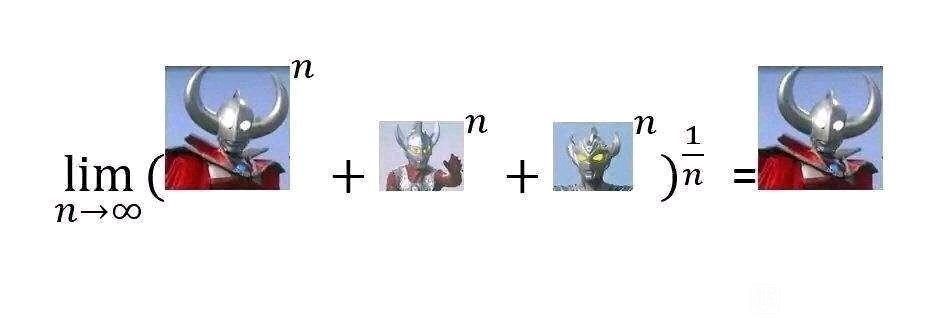
\includegraphics[width=0.7\textwidth]{fig1-1.jpg}
\end{figure}

\begin{example}
\label{ex:ch01-17}
计算$\lim\limits_{x \to 0}|x|\left[\displaystyle\frac{1}{|x|}\right]$.
\end{example}

\begin{analysis}
直观上看，取整函数$y=[x]$与$y=x$的增长速度相当，因为不管$x$多大，二者只相差了一个小数部分. 这对于$n$趋向无穷大时的极限显然是无关紧要的. 在使用夹逼定理时，利用$[x]\le x<[x]+1$进行放缩.
\end{analysis}

\begin{solution}
首先对$\left[\displaystyle\frac{1}{|x|}\right]$进行放缩.由取整函数的性质：
\begin{eq1}
    \frac{1}{|x|}-1 < \left[\frac{1}{|x|}\right] \le \frac{1}{|x|}
\end{eq1}

整条不等式链同时乘以$|x|$：
$$
1-|x|=|x|\left(\displaystyle\frac{1}{|x|}-1\right) < |x|\left[\displaystyle\frac{1}{|x|}\right] \le |x|\left(\displaystyle\frac{1}{|x|}\right)=1
$$

当$x \to 0$时，不等式链最左侧和最右侧的极限都为1. 根据夹逼定理，被夹的$|x|\left[\displaystyle\frac{1}{|x|}\right]$极限也为1.
\end{solution}

\subsubsection{极限相关结论和定理的使用}\par
本节主要讨论一些不能直接计算的极限问题，如求和式的极限（级数）、连乘积、由递推式给出的序列等等. 解决这些问题需要同学们灵活地使用书本上介绍的定理和结论. 在前文中，我们已经将它们全部列出. 希望同学们通过本节所讲的题目，体会这些定理的使用场景和使用方法. \vspace{0.5em}

\textbf{1.~~夹逼定理处理无穷求和}\vspace{0.25em}

遇到无穷求和的极限，最好的情况是利用裂项写出求和的结果，再求极限. 如遇到不能裂项的题目，我们就要考虑使用放缩加上夹逼定理来解决. 先看一道例题：

\begin{example}
\label{ex:ch01-18}
计算$\lim\limits_{n \to \infty}\left( \displaystyle\frac{1}{\sqrt{n^{2}+1}} + \displaystyle\frac{1}{\sqrt{n^{2}+2}} + \cdots +\displaystyle\frac{1}{\sqrt{n^{2}+n}}\right)$.
\end{example}

\begin{solution}
对极限式进行放缩：
\begin{eq1}
    \frac{n}{\sqrt{n^2+n}} < \left( \displaystyle\frac{1}{\sqrt{n^{2}+1}} + \displaystyle\frac{1}{\sqrt{n^{2}+2}} + \cdots +\displaystyle\frac{1}{\sqrt{n^{2}+n}}\right) < \frac{n}{\sqrt{n^2+1}}
\end{eq1}

而$\lim\limits_{n \to \infty}\displaystyle\frac{n}{\sqrt{n^2+n}} = \lim\limits_{n \to \infty}\displaystyle\frac{n}{\sqrt{n^2+1}}=1$.
由夹逼定理：
\begin{eq1}
    \lim\limits_{n \to \infty}\left( \displaystyle\frac{1}{\sqrt{n^{2}+1}} + \displaystyle\frac{1}{\sqrt{n^{2}+2}} + \cdots +\displaystyle\frac{1}{\sqrt{n^{2}+n}}\right)=1
\end{eq1}
\end{solution}

在本题中，
我们将所有的分母$\sqrt{n^{2}+k}$都放缩成了最大值$\sqrt{n^{2}+n}$和最小值$\sqrt{n^{2}+1}$，从而把求和中的每一项都变得相同. 同学们可能第一反应会觉得这样放缩太粗糙了，没想到这样也能成功. 其实，无穷多个无穷小量求和是否收敛，关键要看这个无穷小量的阶数. 将$\displaystyle\frac{1}{\sqrt{n^{2}+k}}$放缩为$\displaystyle\frac{1}{\sqrt{n^{2}+1}}$或$\displaystyle\frac{1}{\sqrt{n^{2}+n}}$，放缩前后是等价无穷小量，对于无穷求和是否收敛是没有影响的. 因此，我们可以把“保持等价无穷小”作为此类放缩的金标准.

\begin{example}
\label{ex:ch01-19}
计算$\lim\limits_{n \to \infty}\left(  \displaystyle\frac{1}{n^2+n+1}+ \displaystyle\frac{2}{n^2+n+2}+ \cdots +\displaystyle\frac{n}{n^2+n+n}\right)$.
\end{example}

\begin{solution}
对极限式进行放缩：
$$
\displaystyle\frac{1+2+\cdots + n}{n^{2}+n+n} <
\left(  \displaystyle\frac{1}{n^2+n+1}+ \displaystyle\frac{2}{n^2+n+2}+ \cdots +\displaystyle\frac{n}{n^2+n+n}\right)
< \displaystyle\frac{1+2+\cdots + n}{n^{2}+n+1}
$$

对左式取极限：
$$
\lim\limits_{n \to \infty}\displaystyle\frac{1+2+\cdots + n}{n^{2}+n+n} =
\limn \displaystyle\frac{n^{2}+n}{2(n^{2}+n+n)} = \frac{1}{2}
$$

对右式取极限：
$$
\lim\limits_{n \to \infty}\displaystyle\frac{1+2+\cdots + n}{n^{2}+n+1} =
\limn \displaystyle\frac{n^{2}+n}{2(n^{2}+n+1)} = \frac{1}{2}
$$

由夹逼定理，$\lim\limits_{n \to \infty}\left(  \displaystyle\frac{1}{n^2+n+1}+ \displaystyle\frac{2}{n^2+n+2}+ \cdots +\displaystyle\frac{n}{n^2+n+n}\right)=\displaystyle\frac{1}{2}$.
\end{solution}

\textbf{2.~~利用无界性证明极限不存在}\vspace{0.25em}

如果一个序列因为趋于无穷而极限不存在，基本上一眼就能看出来，不需要任何技巧. 如果面对如此简单的问题却不会下手写证明，将会非常尴尬.
最简洁的写法是利用“收敛序列必有界”的性质，证明序列没有上界或没有下界.

\begin{example}
\label{ex:ch01-20}
设$x_{n}=n^2$. 证明：序列$\left\{ x_{n} \right\}$极限不存在.
\end{example}

\begin{proof}
任取正数$M$.
 显然，当$n>N=[\sqrt{M}]+1$时，有$x_{n}>M$.
 这说明$\left\{ x_{n} \right\}$无上界，从而$x_{n}$极限不存在.
\end{proof}

\textbf{3.~~利用子列收敛原理证明极限不存在}\vspace{0.5em}

子列收敛原理告诉我们，若一个序列极限是$A$，则任取它的一个子列，它的极限也是$A$. 对于函数的子列也有类似的结论（见1.1.3节）.
反过来说，假设找到了序列的两个子列，它们的极限不同，就可以证明原序列极限不存在.我们先看一个简单的例子，理解它的用法.

\begin{example}
\label{ex:ch01-21}
设$x_{n}=\sin \displaystyle\frac{n\pi}{2}$. 证明：序列$\left\{ x_{n} \right\}$极限不存在.
\end{example}

\begin{proof}
取$\left\{ x_{n} \right\}$的两个子列$\left\{ a_{n} \right\}$和$\left\{ b_{n} \right\}$. 其中，$a_{n}=x_{4n-3}=1$，
$b_{n}=x_{4n-1}=-1$. 显然，$\left\{ a_{n} \right\}$和$\left\{ b_{n} \right\}$的极限分别是$1$和$-1$. 根据子列收敛原理（的逆否命题），序列$\left\{ x_{n} \right\}$极限不存在.
\end{proof}

有同学可能想问：
如果找不到两个极限不同的子列怎么办？这其实不需要担心.
我们可以自信地说：
若序列$\left\{ x_{n} \right\}$有界而且极限不存在，
那么，一定会存在这样的两个极限不同的子列，帮助我们证明$\left\{ x_{n} \right\}$的极限不存在. 不仅如此，还有一个通用办法来的构造这样的两个子列！对于上述序列中的任意一项$x_{n}$，取它之后所有的项，组成的集合记为$X_{n}=\left\{ x_{n+1},~x_{n+2},\cdots \right\} $则$a_{n}=\sup X_{n}$和$b_{n}=\inf X_{n}$就是我们要找的两个子列，且一定有$\lim\limits_{n \to \infty}a_{n}>\lim\limits_{n \to \infty}b_{n}$.
这里$\sup$是指上确界，即最小的上界；$\inf$指下确界，即最大的下界.
可对照上面的例\ref{ex:ch01-21}来理解这个结论.由于这个结论涉及到高数范围之外的定理，在考试时只能作为构造技巧使用，
不能代替证明过程.\vspace{1em}

接下来，作为拓展，我们为大家介绍一类判断极限是否存在的思路——研究相邻两项之比或者相邻两项之差. 这是一个非常具有普适性的思路，也会引出一些好用的“二级结论”（实际上是数学分析中重要的定理）.学有余力的同学可以记下相关的结论和证明方法，在考试时使用；如果没有精力，也可以把这些结论的证明当成练习题. 但是，最关键的是要掌握思想方法. 我们从一个书本中有的定理开始为大家讲解.\vspace{1em}

\textbf{4.~~单调有界原理}\vspace{0.25em}

当一个序列本身很复杂，而相邻两项之比或者之差的形式较简单，我们就应该对此给予关注. 最简单的情况是，我们通过相邻两项作比或者作差，发现序列具有单调性.
这时再配合以有界性，就可以使用单调有界原理了.

\begin{example}
\label{ex:ch01-22}
证明：$a_{n}=\displaystyle\frac{n!}{(2n+1)!!}=\displaystyle\frac{n(n-1)\cdots 3 \cdot 2 \cdot 1}{(2n+1)(2n-1)\cdots 3 \cdot 1}$
的极限为$0$.
\end{example}

\begin{proof}
计算$\left\{ a_{n} \right\}$的相邻两项之比：
$$
\frac{a_{n+1}}{a_{n}} = \frac{(n+1)!}{(2n+3)!!} \cdot \frac{(2n+1)!!}{n!} = \frac{n+1}{2n+3} < 1
$$

即$a_{n+1}<a_{n}$,序列$\left\{ a_{n} \right\}$单调递减. 显然0是$\left\{ a_{n} \right\}$的一个下界. 根据单调有界原理，$\left\{ a_{n} \right\}$收敛.\par
（注意，以上只是证明了极限存在，
还需要再证明极限就是0.）\par

设$\lim\limits_{n \to \infty}a_{n}=a$，对递推式两边同时取极限：
\begin{equation}
    \begin{aligned}
        \lim\limits_{n \to \infty} a_{n+1} = \lim\limits_{n \to \infty}\left( \frac{n+1}{2n+3}a_{n} \right)
        \nonumber
    \end{aligned}
\end{equation}

得到：
$$
a= \frac{1}{2}a
$$

解得$a=0$. 即$\lim\limits_{n \to \infty}a_{n}=0$.
\end{proof}

有一类要使用单调有界原理解决的经典题型：给出序列的递推公式，证明极限存在并计算极限值. 一般来说，解题分为以下3步：（1）证明序列有上界（下界）；
（2）证明序列单调递增（递减），从而极限存在；（3）递推式两边同时取极限，计算极限值. 前两个步骤常用数学归纳法完成.

\begin{example}
\label{ex:ch01-23}
设序列$\left\{ x_{n} \right\}$由递推公式
$x_{n+1}=\displaystyle\frac{1}{2}\left( x_{n}+\displaystyle\frac{1}{x_{n}} \right)$
给出，且$x_{1}>0$. \par
(1)~证明$\left\{ x_{n} \right\}$极限存在，并计算极限值；

(2)~计算：$\lim\limits_{n \to \infty}\displaystyle\frac{1-x_{n+1}}{1-\cos(1-x_{n})}$.
\end{example}

\begin{solution}
(1)~~用数学归纳法易证$x_{n}>0$. 则对任意$n>1$，$x_{n}=\displaystyle\frac{1}{2}\left( x_{n-1}+\displaystyle\frac{1}{x_{n-1}} \right) \ge 1$. 即$1$是$x_{n}$的一个下界. 另外，$x_{n+1}-x_{n}= \displaystyle\frac{1}{2}\left( x_{n}+\displaystyle\frac{1}{x_{n}} \right)-x_{n}
=\displaystyle\frac{1-x_{n}^{2}}{x_{n}} \le 0$. 因此$\left\{ x_{n}\right\}$单调递减. 由单调有界定理可知，$\left\{ x_{n}\right\}$的极限存在.\par
设$\lim\limits_{n \to \infty}x_{n}=X$. 对递推式两边同时取极限：
$$
\lim\limits_{n \to \infty}x_{n+1}= \lim\limits_{n \to \infty}\displaystyle\frac{1}{2}\left( x_{n}+\displaystyle\frac{1}{x_{n}} \right)
$$

得到：
$$
X = \frac{1}{2}\left( X+\frac{1}{X} \right)
$$

解得$X=1$，即$\lim\limits_{n \to \infty}x_{n}=1$.

(2)
\begin{equation}
    \begin{aligned}
        \lim\limits_{n \to \infty}\displaystyle\frac{1-x_{n+1}}{1-\cos(1-x_{n})}
        &= \lim\limits_{n \to \infty}\displaystyle\frac{1-\frac{1}{2}\left( x_{n}+\frac{1}{x_{n}} \right)}{\frac{1}{2}(1-x_{n})^{2}}\\
        &= \lim\limits_{n \to \infty}\displaystyle\frac{2x_{n}-x_{n}^{2}-1}{x_{n}(1-x_{n})^2}\\
        &= 1
        \nonumber
    \end{aligned}
\end{equation}
\end{solution}

从逻辑上讲，我们必须先证明$\left\{ x_{n}\right\}$的极限存在，再求它的极限. 但是为了解题方便，同学们可以先在草稿纸上完成最后一步，即先求出极限的值.
因为极限值可以作为重要的参考，帮助我们猜出序列的上下界或者单调趋势. 例如在上一道例题中，可以先计算出$\left\{ x_{n}\right\}$的极限（若存在则）等于$1$.
而题目给出的首项$x_{1}$是大于$1$的，因此该序列可能是从$1$的上方单调递减趋向于$1$，并且$1$是一个下界. 能够猜到这个程度，用数学归纳法证明出来也就不难了.
如果觉得判断序列的上下界和单调性有困难，可以使用“蛛网图”法辅助判断.

~\par
\textbf{5.~~柯西命题}\vspace{0.5em}

请回顾本讲义中的例\ref{ex:ch01-06}. 在这道题中我们证明了：若序列$\left\{ a_{n}\right\}$的极限为$a$，则其前$n$项的算术平均值极限也为$a$. 接下来，请同学们一起来
尝试证明这个结论对于几何平均值和调和平均值也都成立.

\begin{example}
\label{ex:ch01-24}
设非零序列$\left\{ a_{n}\right\}$的极限为$a$，证明：$\lim\limits_{n \to \infty}\displaystyle\frac{n}{\dfrac{1}{a_{1}}+\dfrac{1}{a_{2}}+\cdots +\dfrac{1}{a_{n}}}=a$.
\end{example}

\begin{proof}
令$b_{n}=\displaystyle\frac{1}{a_{n}}$，则$\lim\limits_{n \to \infty}b_{n}=\displaystyle\frac{1}{a}$. 应用例\ref{ex:ch01-06}的结论：
$$
\lim\limits_{n \to \infty}\displaystyle\frac{n}{\dfrac{1}{a_{1}}+\dfrac{1}{a_{2}}+\cdots +\dfrac{1}{a_{n}}} = \lim\limits_{n \to \infty}\displaystyle\frac{n}{b_{1}+b_{2}+\cdots +b_{n}}=\frac{1}{\lim\limits_{n \to \infty}b_{n}}=a
$$
\end{proof}

\begin{example}
\label{ex:ch01-25}
设正数序列$\left\{ a_{n}\right\}$的极限为$a$. 证明：$\lim\limits_{n \to \infty}\sqrt[n]{a_{1}a_{2}\cdots a_{n}}=a$.
\end{example}

\begin{proof}
利用基本不等式链进行放缩：
$$
\lim\limits_{n \to \infty}\displaystyle\frac{n}{\dfrac{1}{a_{1}}+\dfrac{1}{a_{2}}+\cdots +\dfrac{1}{a_{n}}}
\le \sqrt[n]{a_{1}a_{2}\cdots a_{n}} \le \frac{a_{1}+a_{2}+\cdots +a_{n}}{n}
$$

根据例\ref{ex:ch01-06}和例\ref{ex:ch01-24}结论，左右侧的极限均为$a$. 根据夹逼定理，$\lim\limits_{n \to \infty}\sqrt[n]{a_{1}a_{2}\cdots a_{n}}=a$.
\end{proof}

以上关于算术平均值、几何平均值和调和平均值的结论，合称为\textbf{柯西命题}. 柯西命题的推论很好地利用了序列相邻项之差和相邻项之比所提供的信息. 接下来我们分开讲述这两种不同的处理方式. \par
~\par
\textbf{6.~~相邻项之比的处理——等比数列的启示}\vspace{0.25em}

请回顾本讲义中的例\ref{ex:ch01-22}. 在该题中，我们曾经证到：
$$
\setlength\abovedisplayskip{10pt}
\setlength\belowdisplayskip{10pt}
\frac{a_{n+1}}{a_{n}} = \frac{(n+1)!}{(2n+3)!!} \cdot \frac{(2n+1)!!}{n!} = \frac{n+1}{2n+3}
$$

当时我们使用了单调有界原理，再对递推式两边求极限，才得到$\left\{ a_{n} \right\}$极限为$0$的结论. 其实，有一个更直截了当的说明方式：注意到
$\lim\limits_{n \to \infty}\displaystyle\frac{a_{n+1}}{a_{n}}=\lim\limits_{n \to \infty}\displaystyle\frac{n+1}{2n+3}=\displaystyle\frac{1}{2}$. 换言之，当$n$很大时， $\left\{ a_{n} \right\}$十分接近于公比为$\displaystyle\frac{1}{2}$的等比数列，而公比小于$1$的等比数列一定是收敛于$0$的.
那么，如何严格地证明这一点呢?

\begin{example}
\label{ex:ch01-26}
给定序列$\left\{ a_{n}\right\}$. 若$\lim\limits_{n \to \infty}\left| \displaystyle\frac{a_{n+1}}{a_{n}} \right|=r<1$，证明：$\lim\limits_{n \to \infty}a_{n}=0$.
\end{example}

\begin{proof}
根据极限的保号性（或者直接根据极限的定义），存在正整数$N$，使得当$n>N$时，有$\left| \displaystyle\frac{a_{n+1}}{a_{n}} \right|<\displaystyle\frac{r+1}{2}<1$.\par

则有（这里使用分段处理的技巧）：
\begin{equation}
    \begin{aligned}
        |a_{n}|
        &=  \left| a_{1}\cdot \frac{a_{2}}{a_{1}} \cdot \frac{a_{3}}{a_{2}} \cdots \frac{a_{N+1}}{a_{N}}\right| \cdot \left| \frac{a_{N+2}}{a_{N+1}} \cdots \frac{a_{n}}{a_{n-1}}  \right| \\
        &\le \left| a_{1}\cdot \frac{a_{2}}{a_{1}} \cdot \frac{a_{3}}{a_{2}} \cdots \frac{a_{N+1}}{a_{N}}\right| \cdot \left( \frac{r+1}{2} \right)^{n-N} \to 0~~(n \to \infty)
        \nonumber
    \end{aligned}
\end{equation}

另一方面，$|a_{n}|>0$. 由夹逼定理，$\lim\limits_{n \to \infty}|a_{n}|=0$. 于是$\lim\limits_{n \to \infty}a_{n}=0$.
\end{proof}

若“公比”$r$是任意实数，还有一个更加泛用的命题，它是柯西命题的直接推广：

\begin{example}
\label{ex:ch01-27}
\textbf{柯西命题推论1}\quad 给定正数序列$\left\{ a_{n}\right\}$. 若$\lim\limits_{n \to \infty}  \displaystyle\frac{a_{n+1}}{a_{n}} =a$.
证明：$\lim\limits_{n \to \infty} \sqrt[n]{a_{n}}=a$.
\end{example}

\begin{proof}
将$a_{n}$拆成连乘积的形式：
$$
\lim\limits_{n \to \infty} \sqrt[n]{a_{n}} = \lim\limits_{n \to \infty} \sqrt[n]{a_{1}} \cdot \sqrt[n]{\frac{a_{2}}{a_{1}} \cdot \frac{a_{3}}{a_{2}} \cdots \frac{a_{n}}{a_{n-1}}  }
$$

其中$\lim\limits_{n \to \infty} \sqrt[n]{a_{1}}=1$.根据例\ref{ex:ch01-25}立即得到：$\lim\limits_{n \to \infty} \sqrt[n]{ \displaystyle\frac{a_{2}}{a_{1}} \cdot \displaystyle\frac{a_{3}}{a_{2}} \cdots \frac{a_{n}}{a_{n-1}}}=a$.

因此，$\lim\limits_{n \to \infty} \sqrt[n]{a_{n}}=a$.
\end{proof}

上述结论最大的用途在于处理含有阶乘的数列，因为阶乘在相邻项相除时会抵消得干干净净. 例\ref{ex:ch01-22}即是如此. 我们再给一道这样的例题：

\begin{example}
\label{ex:ch01-28}
计算：$\lim\limits_{n \to \infty}\displaystyle\frac{\sqrt[n]{n!}}{n} $.
\end{example}

\begin{analysis}
要求的极限含有$n$次根号，根号下有阶乘. 因此，把根号下的部分看成命题中的$a_{n}$.
\end{analysis}

\begin{solution}
令$a_{n} = \displaystyle\frac{n!}{n^{n}}$. 计算相邻两项之比的极限：\par
\begin{equation}
    \begin{aligned}
        \lim\limits_{n \to \infty}\frac{a_{n+1}}{a_{n}}
        &= \lim\limits_{n \to \infty} \frac{(n+1)!}{(n+1)^{n+1}} \cdot \frac{n^{n}}{n!} \\
        &= \lim\limits_{n \to \infty} \frac{n^{n}}{(n+1)^{n}}\\
        &= \lim\limits_{n \to \infty} \left( 1-\frac{1}{n-1}  \right)^{n}\\
        &= e^{-1}
        \nonumber
    \end{aligned}
\end{equation}
\par
根据刚才介绍的命题，$\lim\limits_{n \to \infty}\displaystyle\frac{\sqrt[n]{n!}}{n} = \lim\limits_{n \to \infty} \sqrt[n]{a_{n}}= \lim\limits_{n \to \infty}  \displaystyle\frac{a_{n+1}}{a_{n}} = e^{-1}$.
\end{solution}

\textbf{7.~~相邻项之差的处理——Stolz定理}\vspace{0.25em}

对于相邻两项之差，也有和上面类似的推论：

\begin{example}
\label{ex:ch01-29}
\textbf{柯西命题推论2}\quad 给定序列$\left\{ a_{n}\right\}$. 若$\lim\limits_{n \to \infty} (a_{n+1}-a_{n})=a$. 证明：$\lim\limits_{n \to \infty} \displaystyle\frac{a_{n}}{n}=a$.
\end{example}

\begin{proof}
将$a_{n}$拆成求和的形式：
$$
\lim\limits_{n \to \infty}  \displaystyle\frac{a_{n}}{n} =
\lim\limits_{n \to \infty} \left[ \frac{a_{1}}{n} + \frac{(a_{2}-a_{1}) + (a_{3}-a_{2})+ \cdots +(a_{n}-a_{n-1})}{n} \right]
$$

其中，$\lim\limits_{n \to \infty}\displaystyle\frac{a_{1}}{n}=0$，而根据算术平均值形式的柯西命题（例\ref{ex:ch01-06}）立即得到：
$$
\lim\limits_{n \to \infty} \displaystyle\frac{(a_{2}-a_{1}) + (a_{3}-a_{2})+ \cdots +(a_{n}-a_{n-1})}{n}=a.
$$
\par
因此，$\lim\limits_{n \to \infty} \displaystyle\frac{a_{n}}{n}=a$.
\end{proof}

关于这个命题，我们不给例题. 因为有一个更好用的“大杀器”推荐给同学们，它叫做Stolz定理. 这个定理的证明本身也可以作为一道例题：

\begin{example}
\label{ex:ch01-30}
\textbf{Stolz定理}\quad 证明：设序列$\left\{ y_{n} \right\}$严格单调递增且趋于正无穷，$\lim\limits_{n \to \infty} \displaystyle\frac{x_{n}-x_{n-1}}{y_{n}-y_{n-1}}=a$（$a$既可以是有限值，也可以是正无穷或负无穷）,则$\lim\limits_{n \to \infty} \displaystyle\frac{x_{n}}{y_{n}}=a$.
\end{example}

\begin{proof}
先考虑$a=0$的情况.
由$\lim\limits_{n \to \infty} \displaystyle\frac{x_{n}-x_{n-1}}{y_{n}-y_{n-1}}=0$，可知对任意$\epsilon>0$，存在正整数$N_{1}$，使得当$n>N_{1}$时，有$|x_{n}-x_{n-1}|<\epsilon$. 由于$y_{n}$是正无穷大量，不妨设$y_{N_{1}}>0$，于是：

\begin{equation}
    \begin{aligned}
        |x_{n}-x_{N_{1}}|
        &\le |x_{n}-x_{n-1}|+|x_{n-1}-x_{n-2}|+ \cdots +|x_{N_{1}+1}-x_{N_{1}}| \\
        &< \epsilon(y_{n}-y_{n-1})+\epsilon(y_{n-1}-y_{n-2})+ \cdots +\epsilon(y_{N_{1}+1}-y_{N_{1}}) \\
        &= \epsilon(y_{n}-y_{N_{1}})
        \nonumber
    \end{aligned}
\end{equation}\par
不等式两边同时除以$y_{n}$：
$$
\left| \frac{x_{n}}{y_{n}} - \frac{x_{N_{1}}}{y_{n}}\right|
\le \epsilon \left( 1-\frac{y_{N_{1}}}{y_{n}} \right)
<\epsilon
$$

对于给定的$N_{1}$，存在正整数$N>N_{1}$，使得当$n>N$时，有$\left| \displaystyle\frac{x_{N_{1}}}{y_{n}}\right|<\epsilon$. 从而$\left|\displaystyle\frac{x_{n}}{y_{n}} \right|< \epsilon + \left| \displaystyle\frac{x_{N_{1}}}{y_{n}}\right| <2\epsilon $. 这就证明了$a=0$的情况.

当$a\ne 0$且为有限值时，令$X_{n}=x_{n}-ay_{n}$，于是：
$$
\lim\limits_{n \to \infty} \frac{X_{n}-X_{n-1}}{y_{n}-y_{n-1}} =
\lim\limits_{n \to \infty} \frac{x_{n}-x_{n-1}}{y_{n}-y_{n-1}} -a = 0
$$

则由刚才证过的情况，得到$\lim\limits_{n \to \infty}\displaystyle\frac{X_{n}}{y_{n}}=0$. 从而$\lim\limits_{n \to \infty}\displaystyle\frac{x_{n}}{y_{n}}= \lim\limits_{n \to \infty}\displaystyle\frac{X_{n}}{y_{n}}+a=a$.

对于$a$为正无穷（$a$为负无穷的证明完全类似）的情况，存在正整数$N$，使得当$n>N$时，有$\displaystyle\frac{x_{n}-x_{n-1}}{y_{n}-y_{n-1}}>1$，即$x_{n}-x_{n-1}>y_{n}-y_{n-1}>0$，因此序列$\left\{ x_{n} \right\}$也是单调递增的，而且增长速度快于$\left\{ y_{n} \right\}$，因此$x_{n}$也趋向正无穷. 由之前证明过的情况，得到：
$$
\lim\limits_{n \to \infty}\frac{y_{n}}{x_{n}} =
\lim\limits_{n \to \infty} \frac{y_{n}-y_{n-1}}{x_{n}-x_{n-1}} =0
$$\par
从而$\lim\limits_{n \to \infty} \displaystyle\frac{x_{n}}{y_{n}}=+\infty$.
\end{proof}

从形式上看，Stolz定理是数列版的洛必达法则，只是把导数改为了相邻项之差（称为差分）. 江湖上流传着“遇事不决洛必达”的说法，实际上，“遇事不决Stolz”也未尝不可.

\begin{example}
\label{ex:ch01-31}
用Stolz定理证明：$\lim\limits_{n \to \infty}\displaystyle\frac{\ln n}{n}=0$.
\end{example}

\begin{proof}
直接使用Stolz定理：
\begin{equation}
    \begin{aligned}
        \lim\limits_{n \to \infty}\frac{\ln n}{n}
        &= \lim\limits_{n \to \infty}\frac{\ln n - \ln (n-1)}{n-(n-1)} \\
        &= \lim\limits_{n \to \infty}\ln\left(\frac{n}{n-1} \right) \\
        &= 0
        \nonumber
    \end{aligned}
\end{equation}
\end{proof}

\begin{example}
\label{ex:ch01-32}
用Stolz定理证明：$\lim\limits_{n \to \infty}\displaystyle\frac{n^{k}}{a^{n}}=0$.其中$a>1$，$k$是正整数.
\end{example}

\begin{proof}
直接使用Stolz定理：
\begin{equation}
    \begin{aligned}
        \lim\limits_{n \to \infty}\frac{n^{k}}{a^{n}}
        &= \lim\limits_{n \to \infty}\frac{n^{k}-(n-1)^{k}}{a^{n}-a^{n-1}} \\
        &= \lim\limits_{n \to \infty}\frac{n^{k}-n^{k} +kn^{k-1}-\frac{k(k-1)}{2}n^{k-2}+\cdots}{(a-1)a^{n-1}} \\
        &= \lim\limits_{n \to \infty}\frac{kn^{k-1}}{(a-1)a^{n-1}}
        \nonumber
    \end{aligned}
\end{equation}\par
再对得到的极限式连续使用$k-1$次Stolz定理（这个做法很像连续多次洛必达），得到：
\begin{equation}
    \begin{aligned}
        \lim\limits_{n \to \infty}\frac{n^{k}}{a^{n}}
        &= \frac{k}{a-1}\cdot \lim\limits_{n \to \infty}\frac{n^{k-1}}{a^{n-1}}\\
        &= \frac{k(k-1)}{(a-1)^2}\cdot \lim\limits_{n \to \infty}\frac{n^{k-2}}{a^{n-2}}\\
        ~~~~&\cdots\\
        &= \frac{k!}{(a-1)^k} \cdot \lim\limits_{n \to \infty}\frac{n^{0}}{a^{n-k}}\\
        &= 0
        \nonumber
    \end{aligned}
\end{equation}
\end{proof}

对于含有无穷求和的分式，Stolz定理尤其好用.

\begin{example}
\label{ex:ch01-33}
设$\lim\limits_{n \to \infty}a_{n}=a$. 计算：$\lim\limits_{n \to \infty}\displaystyle\frac{a_{1}+2a_{2}+\cdots +na_{n}}{n^{2}}$.
\end{example}

\begin{solution}
令$x_{n}=a_{1}+2a_{2}+\cdots +na_{n}$，$y_{n}=n^{2}$，由Stolz定理:
\begin{equation}
    \begin{aligned}
        \lim\limits_{n \to \infty}\displaystyle\frac{a_{1}+2a_{2}+\cdots +na_{n}}{n^{2}}
        &= \lim\limits_{n \to \infty}\frac{x_{n}-x_{n-1}}{y_{n}-y_{n-1}}\\
        &= \lim\limits_{n \to \infty} \frac{na_{n}}{n^{2}-(n-1)^{2}}\\
        &= \lim\limits_{n \to \infty} \frac{na_{n}}{2n-1}\\
        &= \frac{a}{2}
        \nonumber
    \end{aligned}
\end{equation}
\end{solution}

\begin{example}
\label{ex:ch01-34}
计算：$\lim\limits_{n \to \infty}\displaystyle\frac{1^{k}+2^{k}+\cdots +n^{k}}{n^{k+1}}$.其中$k$为正整数.
\end{example}

\begin{solution}
令$x_{n}=1^{k}+2^{k}+\cdots +n^{k}$，$y_{n}=n^{k+1}$，由Stolz定理：

\begin{equation}
    \begin{aligned}
        \lim\limits_{n \to \infty}\displaystyle\frac{1^{k}+2^{k}+\cdots +n^{k}}{n^{k+1}}
        &= \lim\limits_{n \to \infty}\frac{x_{n}-x_{n-1}}{y_{n}-y_{n-1}}\\
        &= \lim\limits_{n \to \infty}\frac{n^{k}}{n^{k+1}-(n-1)^{k+1}}\\
        &= \lim\limits_{n \to \infty}\frac{n^{k}}{n^{k+1}-n^{k+1}+(k+1)n^{k}-\frac{k(k+1)}{2}n^{k-1}+\cdots}\\
        &= \lim\limits_{n \to \infty}\frac{n^{k}}{(k+1)n^{k}} \\
        &= \frac{1}{k+1}
        \nonumber
    \end{aligned}
\end{equation}
\end{solution}

\subsubsection{间断点的判断}\par
给定一个函数，求问间断点的个数，或者第一类/第二类间断点的个数. 一般来说，题目中的函数是由一些初等函数的复合给出.
此时，函数的间断点基本只出现在：（1）无定义的点，尤其是分母为0的点；（2）绝对值符号中为0的点.
接下来，无非是计算这些点处的左右极限. 建议同学们逐点把左右极限计算清楚再下定论，不要害怕繁琐的题目.\par
~\par

\setstretch{2.25}

\begin{example}
\label{ex:ch01-35}
函数$f(x)=\displaystyle\frac{\left( e^{\frac{1}{x-1}}-1 \right)|x|}{(x+1)\ln|x-1|}$有多少间断点？有多少第一类间断点？
\end{example}

\begin{solution}
$f(x)$的间断点为$x=-1,1,0,2$，共有4个.\par
对于$x=-1$，$\lim\limits_{x \to -1}f(x)= \lim\limits_{x \to -1} \displaystyle\frac{e^{-\frac{1}{2}}-1}{(x+1)\ln 2} =\infty$. 从而$x=-1$是第二类间断点（无穷间断点）.\par
对于$x=0$，$\lim\limits_{x \to 0^{+}}f(x)=\lim\limits_{x \to 0^{+}}\displaystyle\frac{x(e^{-1}-1)}{\ln(1-x)}=1-e^{-1}$;
  $\lim\limits_{x \to 0^{-}}f(x)=\lim\limits_{x \to 0^{-}}\displaystyle\frac{-x(e^{-1}-1)}{\ln(1-x)}=e^{-1}-1$. 从而$x=0$是第一类间断点（跳跃间断点）.\par
对于$x=1$,$\lim\limits_{x \to 1^{+}}f(x) = \lim\limits_{x \to 1^{+}} \displaystyle\frac{e^{\frac{1}{x-1}}-1}{2\ln(x-1)}$.令$u=\displaystyle\frac{1}{x-1}$. 则$\lim\limits_{x \to 1^{+}}f(x) = \lim\limits_{u \to +\infty}\displaystyle\frac{e^{u}-1}{-2\ln u}=\infty$. 从而$x=1$是第二类间断点（无穷间断点）.\par
对于$x=2$，$\lim\limits_{x \to 2}f(x) = \lim\limits_{x \to 2}\displaystyle\frac{2(e-1)}{3\ln|x-1|}=\infty$. 从而$x=2$是第二类间断点（无穷间断点）.\par
综上，$f(x)$的第一类间断点为$x=0$，仅有1个.
\end{solution}

\setstretch{1.75}
